\chapter{Ergebnisse}

Die Klassifizierung des Zustandes der menschlichen Retina anhand von OCT
Aufnahmen in 4 Klassen (gesund + 3 Erkrankungen) lässt sich mit Hilfe des
maschinellen Lernens mit einer Genauigkeit von bis zu $\SI{90}{\percent}$
durchführen. Eine Lösung dieser Aufgabe, wie sie in dieser Arbeit beschrieben
ist, erfordert allerdings eine sehr hohe Rechenkapazität. Der verwendete
Datensatz liefert mit etwa $90\,000$ Bildern in sehr guter Auflösung eine
ausreichende Statistik, um gute Ergebnisse zu erzielen.
Die Hauptarchitektur eines CNN zeigt hierbei mit Abstand die beste
\textit{performance}. Nach etwa 40 Epochen lässt sich mit diesem Netz ein
Modell generieren, welches 4 Klassen mit einer Genauigkeit von
$\SI{90}{\percent}$ unterscheiden kann. Durch die Architektur können so Bilder
verschiedener Größen und Datensätze unterschiedlicher Verteilungen zur
Vorhersage verwendet werden. Durch ausreichende Regularisierung treten keine
Effekte von \textit{overtraining} auf, wie in Abbildung~\ref{fig:hist}


Allerdings lässt sich auch mit deutlich einfacheren Modellen
\begin{figure}
  \subcaptionbox{\textit{accuracy history}}{\centering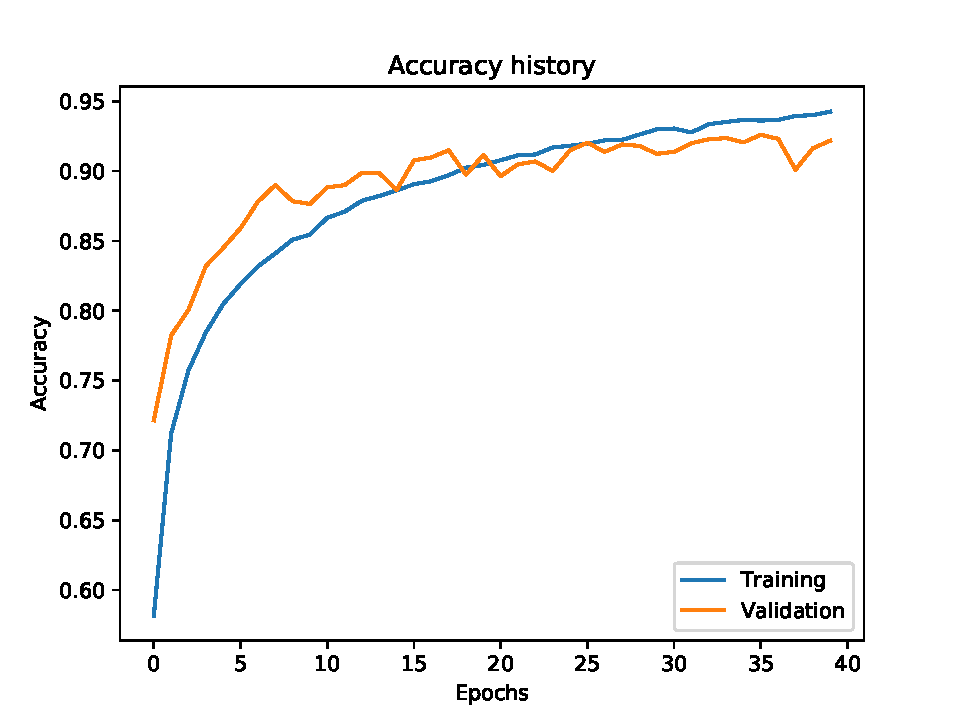
\includegraphics[width=0.48\linewidth]{Plots/accuracy_history_smaller.pdf}}
  \subcaptionbox{\textit{loss history}}{\centering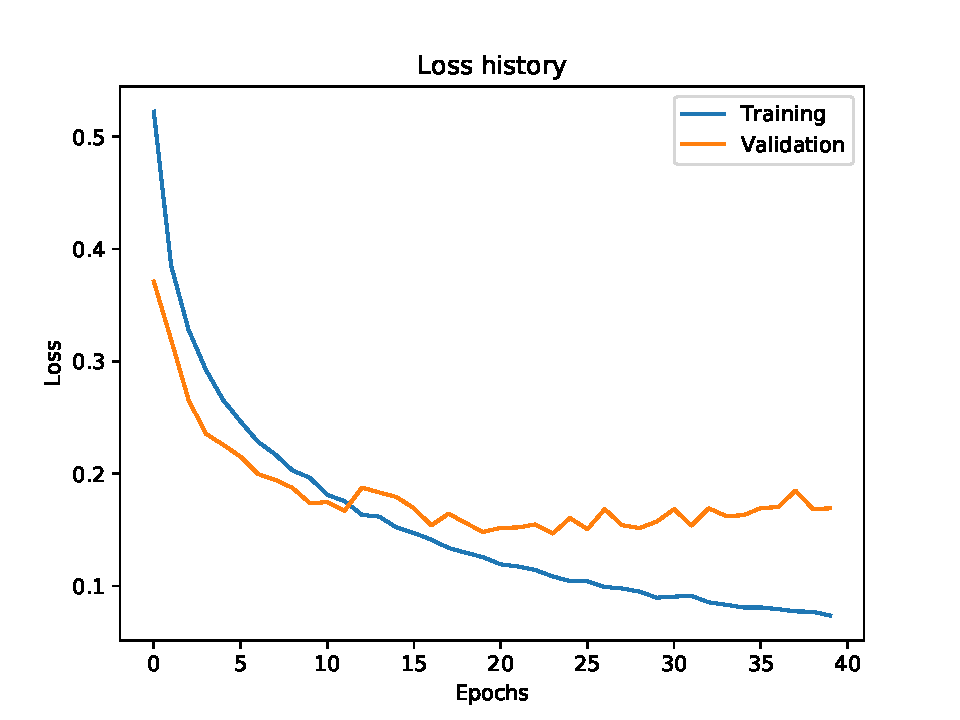
\includegraphics[width=0.48\linewidth]{Plots/loss_history_smaller.pdf}}
  \subcaptionbox{}{\centering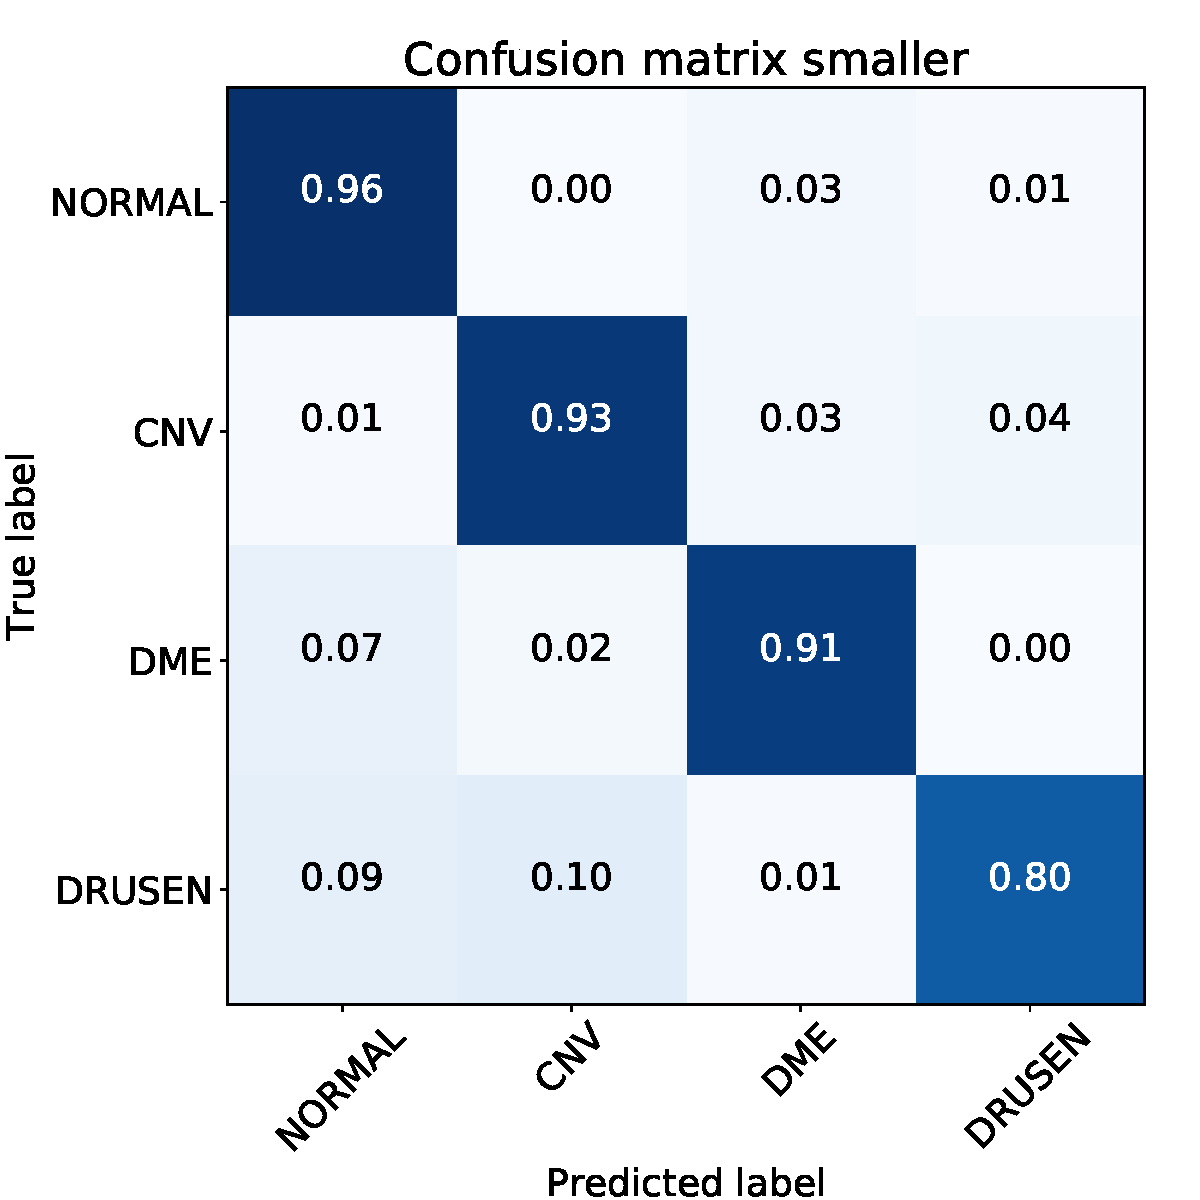
\includegraphics[width=0.48\linewidth]{Plots/confusion_matrix_smaller.pdf}}
  \subcaptionbox{}{\centering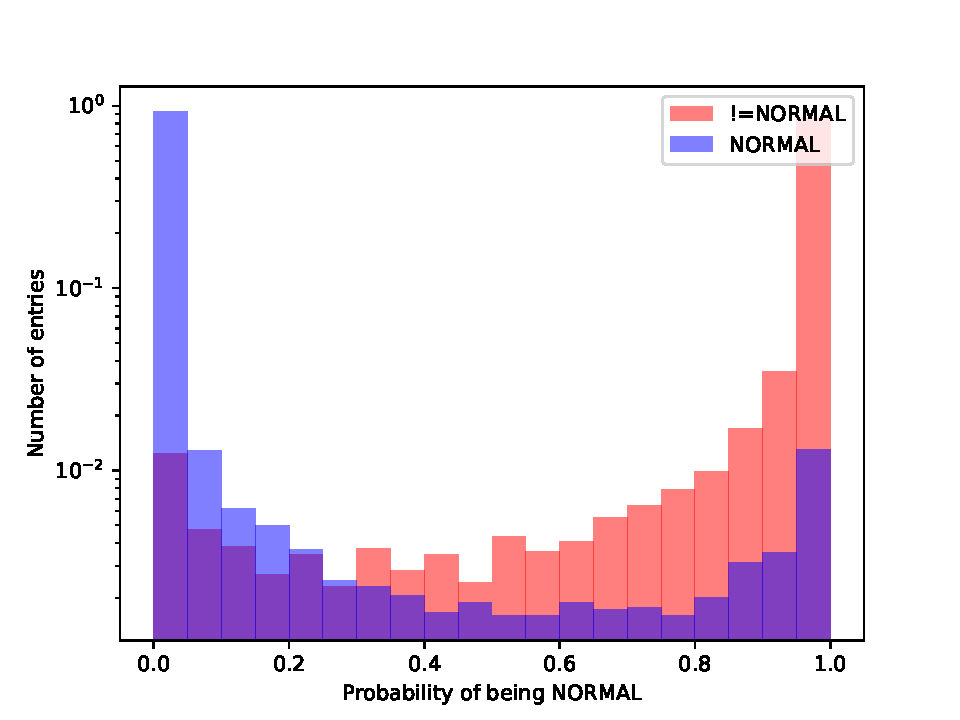
\includegraphics[width=0.5\linewidth]{Plots/NORMAL_or_not_log_smaller.pdf}}
  \caption{Die \textit{accuracy history}, sowie die \textit{loss history} der Hauptarchitektur des CNN. Es zeigen sich hier nach 40 Epochen keine Anzeichen für ein \textit{overtraining}.}
  \label{fig:hist}
\end{figure}
